\documentclass[11pt,a4paper]{article}

\usepackage[margin=0.62in]{geometry}
\usepackage{fontspec}
\usepackage{graphicx}
\usepackage{booktabs}
\usepackage{tabularx}
\usepackage{array}
\usepackage{float}
\usepackage{enumitem}
\usepackage{caption}
\usepackage{titlesec}
\usepackage{xcolor}
\usepackage{hyperref}
\usepackage{lastpage}

\setmainfont{Times New Roman}
\setsansfont{Arial}
\hypersetup{colorlinks=true, linkcolor=black, citecolor=black, urlcolor=blue}
\graphicspath{{figures/}}
\setlength{\parindent}{0pt}
\setlength{\parskip}{3pt}
\sloppy
\setlist[itemize]{leftmargin=1.25em, itemsep=1pt, topsep=2pt}
\setlist[enumerate]{leftmargin=1.35em, itemsep=1pt, topsep=2pt}
\renewcommand{\arraystretch}{1.12}
\captionsetup{font=small, labelfont=bf}
\titleformat{\section}{\large\bfseries}{\thesection}{0.6em}{}
\titleformat{\subsection}{\normalsize\bfseries}{\thesubsection}{0.6em}{}
\titleformat{\subsubsection}{\normalsize\itshape}{\thesubsubsection}{0.6em}{}

\newcolumntype{Y}{>{\raggedright\arraybackslash}X}
\newcommand{\figref}[1]{Fig.~\ref{#1}}

\begin{document}

\begin{titlepage}
\centering
\vspace*{1.0cm}
{\Large\bfseries Student Complaint and Feedback Management System\par}
\vspace{0.4cm}
{\large Project Documentation and OOAD Report\par}
\vspace{0.6cm}
{\normalsize Prepared for Project Documentation Assessment\par}
\vspace{0.9cm}
\begin{tabular}{rl}
Course: & CPS 3962\\
Instructor: & Waqar Ali\\
Project type: & Full-stack course project prototype\\
Backend: & Java Spring Boot 3, Spring Security, Spring Data JPA\\
Frontend: & Vue 3, Vite, Element Plus\\
Database: & H2 for development and MySQL for deployment\\
Documentation date: & June 6, 2026\\
\end{tabular}
\vspace{0.8cm}

\begin{tabular}{rl}
Group members: & Zihao Xu -- 1305978\\
& Zixuan Feng -- 1305979\\
& Zile Ye -- 1306062\\
& Yansong Wen -- 1308070\\
University / Department: & Wenzhou-Kean University, Department of Computer Science and Technology\\
Submission date: & June 6, 2026\\
\end{tabular}
\vfill
{\small This report is limited to the designed and implemented prototype. It does not claim production-level campus deployment readiness.}
\end{titlepage}

\section{Introduction, Problem Statement, Aims, and Objectives}

\subsection{Background of the selected problem}
Universities need a reliable way to receive, classify, assign and monitor student complaints and feedback. In many student-service settings, complaints are still handled through emails, verbal reports, paper forms or informal messaging channels. These channels may work for small volumes, but they make it difficult to trace ownership, preserve evidence, measure response time or confirm whether the student is satisfied with the final resolution.

The proposed Student Complaint and Feedback Management System addresses this problem through a web-based case management prototype. It supports students, anonymous users, student affairs officers, department staff and administrators. The system combines complaint submission, anonymous tracking, department assignment, status logs, SLA signals, notifications, audit logs and reports into one workflow. The design follows object-oriented analysis and design (OOAD) principles and uses UML models as specified by the Object Management Group UML standard \cite{OMG2017UML}.

\subsection{Existing issues or limitations}
The problem analysis identified several limitations in traditional complaint handling:
\begin{itemize}
  \item Complaints may be lost or delayed because there is no central case number or traceable workflow.
  \item Students may not know which department is responsible for handling a complaint.
  \item Staff may lack visibility into overdue, urgent, anonymous or reopened cases.
  \item Evidence files and follow-up messages may be separated from the original complaint.
  \item Administrators may lack reliable audit logs and weekly summaries for management review.
  \item Anonymous reporting is difficult to support when the system must protect identity but still allow status tracking.
\end{itemize}

\subsection{Need for the proposed system}
The proposed system is needed to formalize complaint handling as a transparent case lifecycle. A submitted complaint becomes a \texttt{ComplaintCase} with a unique case number, category, priority, status, due date and related workflow records. Students can track cases and provide additional information. Officers can review, request clarification, assign departments and close cases. Department staff can update progress and mark cases resolved. Administrators can configure reference data, manage accounts, inspect audit logs and generate reports.

\subsection{Core problem statement}
The core problem is: \textit{How can a university prototype provide a structured, role-based and traceable workflow for receiving, assigning, processing and evaluating student complaints and feedback while supporting anonymous submissions and OOAD-based system design?}

\subsection{Project aims}
The main aim is to design and implement a course-project prototype that demonstrates a complete complaint and feedback workflow using modern web technologies and OOAD modeling artifacts.

\subsection{Specific objectives}
\begin{enumerate}
  \item Provide role-based access for students, anonymous users, student affairs officers, department staff and administrators.
  \item Allow authenticated and anonymous complaint submission with category, priority, description and optional attachments.
  \item Generate case numbers and anonymous tracking codes while storing only tracking-code hashes.
  \item Support officer review, information requests, department assignment, department progress updates, resolution and case closure.
  \item Record case messages, status logs, private notes, notifications, audit logs and reports.
  \item Provide system administration for users, departments, categories, permissions, reports and settings.
  \item Demonstrate OOAD concepts through use-case, class, activity, sequence, architecture, ER and navigation diagrams.
  \item Evaluate the prototype through functional tests, role-level validation and observed implementation limitations.
\end{enumerate}

\section{Methodology and Analysis Approach}

\subsection{Adopted methodology and rationale}
The project adopted an iterative and incremental development approach. This choice was appropriate because the system combines several interacting workflows: authentication, complaint submission, anonymous tracking, officer review, department processing, notifications, reporting and administration. An iterative approach allowed the team to model the main workflow first, implement a working vertical slice, then refine role-specific behavior and edge cases. The approach is consistent with modern iterative delivery guidance that emphasizes transparency, inspection, adaptation and working increments \cite{ScrumGuide2020}.

For analysis and design, the project used OOAD. The domain was decomposed into actors, use cases, domain classes, workflow states, sequence interactions and persistent entities. The requirements section was structured with reference to requirements engineering practice, where requirements should be identifiable, verifiable and connected to system functions \cite{ISO29148}.

\subsection{Application during analysis and design}
The analysis started from stakeholder roles and major complaint scenarios. Each scenario was converted into use cases and then mapped to objects. For example, "submit complaint" maps to \texttt{ComplaintCase}, \texttt{Category}, \texttt{CaseAttachment}, \texttt{CaseStatusLog} and \texttt{Notification}. Officer assignment maps to \texttt{Department}, \texttt{CaseAssignment} and status changes. Anonymous tracking maps to \texttt{trackingCodeHash} and public lookup functions.

The same design logic was then reflected in the implementation. The backend uses Spring Boot controllers, services, repositories and JPA domain entities. The frontend uses Vue pages, role-based navigation and API calls. The database schema follows modern relational database design practice, separating persistent data into tables, keys and relationships \cite{DatabaseConcepts2019}.

\subsection{Major development phases}
\begin{table}[H]
\centering
\small
\begin{tabularx}{\textwidth}{p{0.21\textwidth}Y}
\toprule
Phase & Main activities and outputs\\
\midrule
Problem analysis & Identified complaint-handling limitations, target users and expected workflow boundaries.\\
Requirement analysis & Defined functional, non-functional, data, security and deployment requirements.\\
OOAD modeling & Produced use-case, class, activity, sequence, architecture, ER and role navigation diagrams.\\
Backend development & Implemented Spring Boot REST APIs, security, domain services, repositories and tests.\\
Frontend development & Implemented Vue role dashboards, forms, case views, notification presentation and navigation.\\
Evaluation & Ran backend and frontend tests, checked main workflows, identified limits and future improvements.\\
\bottomrule
\end{tabularx}
\caption{Methodology phases followed in the project.}
\end{table}

\section{Requirements Analysis}

\subsection{Stakeholders and actors}
The system supports five actor categories: Student, Anonymous User, Student Affairs Officer, Department Staff and Admin. Students submit and track cases. Anonymous users submit public complaints without logging in and track them with a case number and tracking code. Officers classify, request more information, assign and close cases. Department staff process assigned cases. Admins configure users, departments, categories, reports, audit logs and system settings.

\subsection{Functional requirements}
\begin{table}[H]
\centering
\small
\begin{tabularx}{\textwidth}{p{0.12\textwidth}p{0.22\textwidth}Y}
\toprule
ID & Category & Requirement\\
\midrule
FR1 & Authentication & The system shall allow prototype users to register and log in with JWT-based sessions. University SSO may be integrated in a future deployment.\\
FR2 & Role access & The system shall restrict functions according to Student, Officer, Department Staff and Admin roles.\\
FR3 & Case submission & The system shall allow students to submit complaints or feedback with category, title, description, priority and attachments.\\
FR4 & Anonymous case & The system shall allow public anonymous submission only when the selected category permits anonymity.\\
FR5 & Tracking & The system shall generate a case number and, for anonymous cases, a one-time tracking code.\\
FR6 & Officer workflow & Officers shall review, classify, request additional information, assign departments and close cases.\\
FR7 & Department workflow & Department staff shall view assigned cases, update progress, provide responses and mark cases resolved.\\
FR8 & Notifications & The system shall create in-app notifications for submission, assignment, information request, progress, resolution and closure events.\\
FR9 & Administration & Admins shall manage users, departments, categories, permissions, reports, audit logs and settings.\\
FR10 & Reporting & The system shall provide weekly and summary reports by status, category, department and SLA condition.\\
\bottomrule
\end{tabularx}
\caption{Functional requirements.}
\end{table}

\subsection{Non-functional requirements}
\begin{table}[H]
\centering
\small
\begin{tabularx}{\textwidth}{p{0.18\textwidth}Y}
\toprule
Category & Requirement\\
\midrule
Security & Passwords shall be stored with BCrypt. Role-based endpoint protection shall be enforced by Spring Security.\\
Usability & The frontend shall provide role-specific navigation and clear next actions for each user type.\\
Reliability & Email sending failure shall not block the main complaint workflow. Notification records shall still be stored.\\
Maintainability & Backend logic shall be separated into controllers, services, repositories and domain entities.\\
Traceability & Important workflow actions shall create status logs, notifications or audit records.\\
Portability & The backend shall support H2 for local development and MySQL for deployment.\\
Scalability boundary & The prototype shall support course demonstration workflows, but it shall not claim production-level concurrency.\\
\bottomrule
\end{tabularx}
\caption{Non-functional requirements.}
\end{table}

\subsection{Data and security requirements}
The system must persist users, departments, categories, cases, attachments, messages, status logs, assignments, private notes, notifications, audit logs, weekly reports and system settings. Sensitive credentials are not stored as plain text. Anonymous tracking codes are displayed once and only their hash is stored. Evidence files are stored locally in the prototype, but production use should replace local storage with object storage.

\subsection{Requirement validation criteria}
Each requirement was connected to at least one role, API endpoint, domain entity or frontend workflow. The implemented test suite provides automated validation for case notification flow, category policy, profile updates, settings, SLA policy, tracking code generation, case number generation and frontend presentation logic.

\section{System Design and Modeling}

\subsection{System architecture}
The architecture diagram in \figref{fig:architecture} explains how actors interact with the Vue frontend, how the API client communicates with the Spring Boot backend and how backend services use persistence, file storage, email and optional SSO services. The diagram connects the implementation structure to the analysis decision that user roles should be separated from backend workflow responsibilities.

\begin{figure}[H]
\centering
  
\includegraphics[width=0.94\textwidth,height=0.74\textheight,keepaspectratio]{figure1_system_architecture.png}
\caption{System architecture diagram.}
\label{fig:architecture}
\end{figure}

\subsection{Use-case modeling}
The use-case diagram in \figref{fig:usecase} shows the system from the user's perspective. The Student actor performs login, submission, upload, tracking and follow-up review. The Anonymous User submits and tracks anonymous cases. The Student Affairs Officer reviews, classifies, requests information, assigns departments, closes cases and views reports. Department Staff work on assigned cases. Admin manages accounts, reference data, reports, logs and settings.

The include relationships clarify reusable system functions. For example, complaint submission includes validation and case-number generation. Anonymous submission includes tracking-code generation. This avoids the incorrect assumption that assignment is always part of submission; assignment is an officer action after review.

\begin{figure}[H]
\centering
  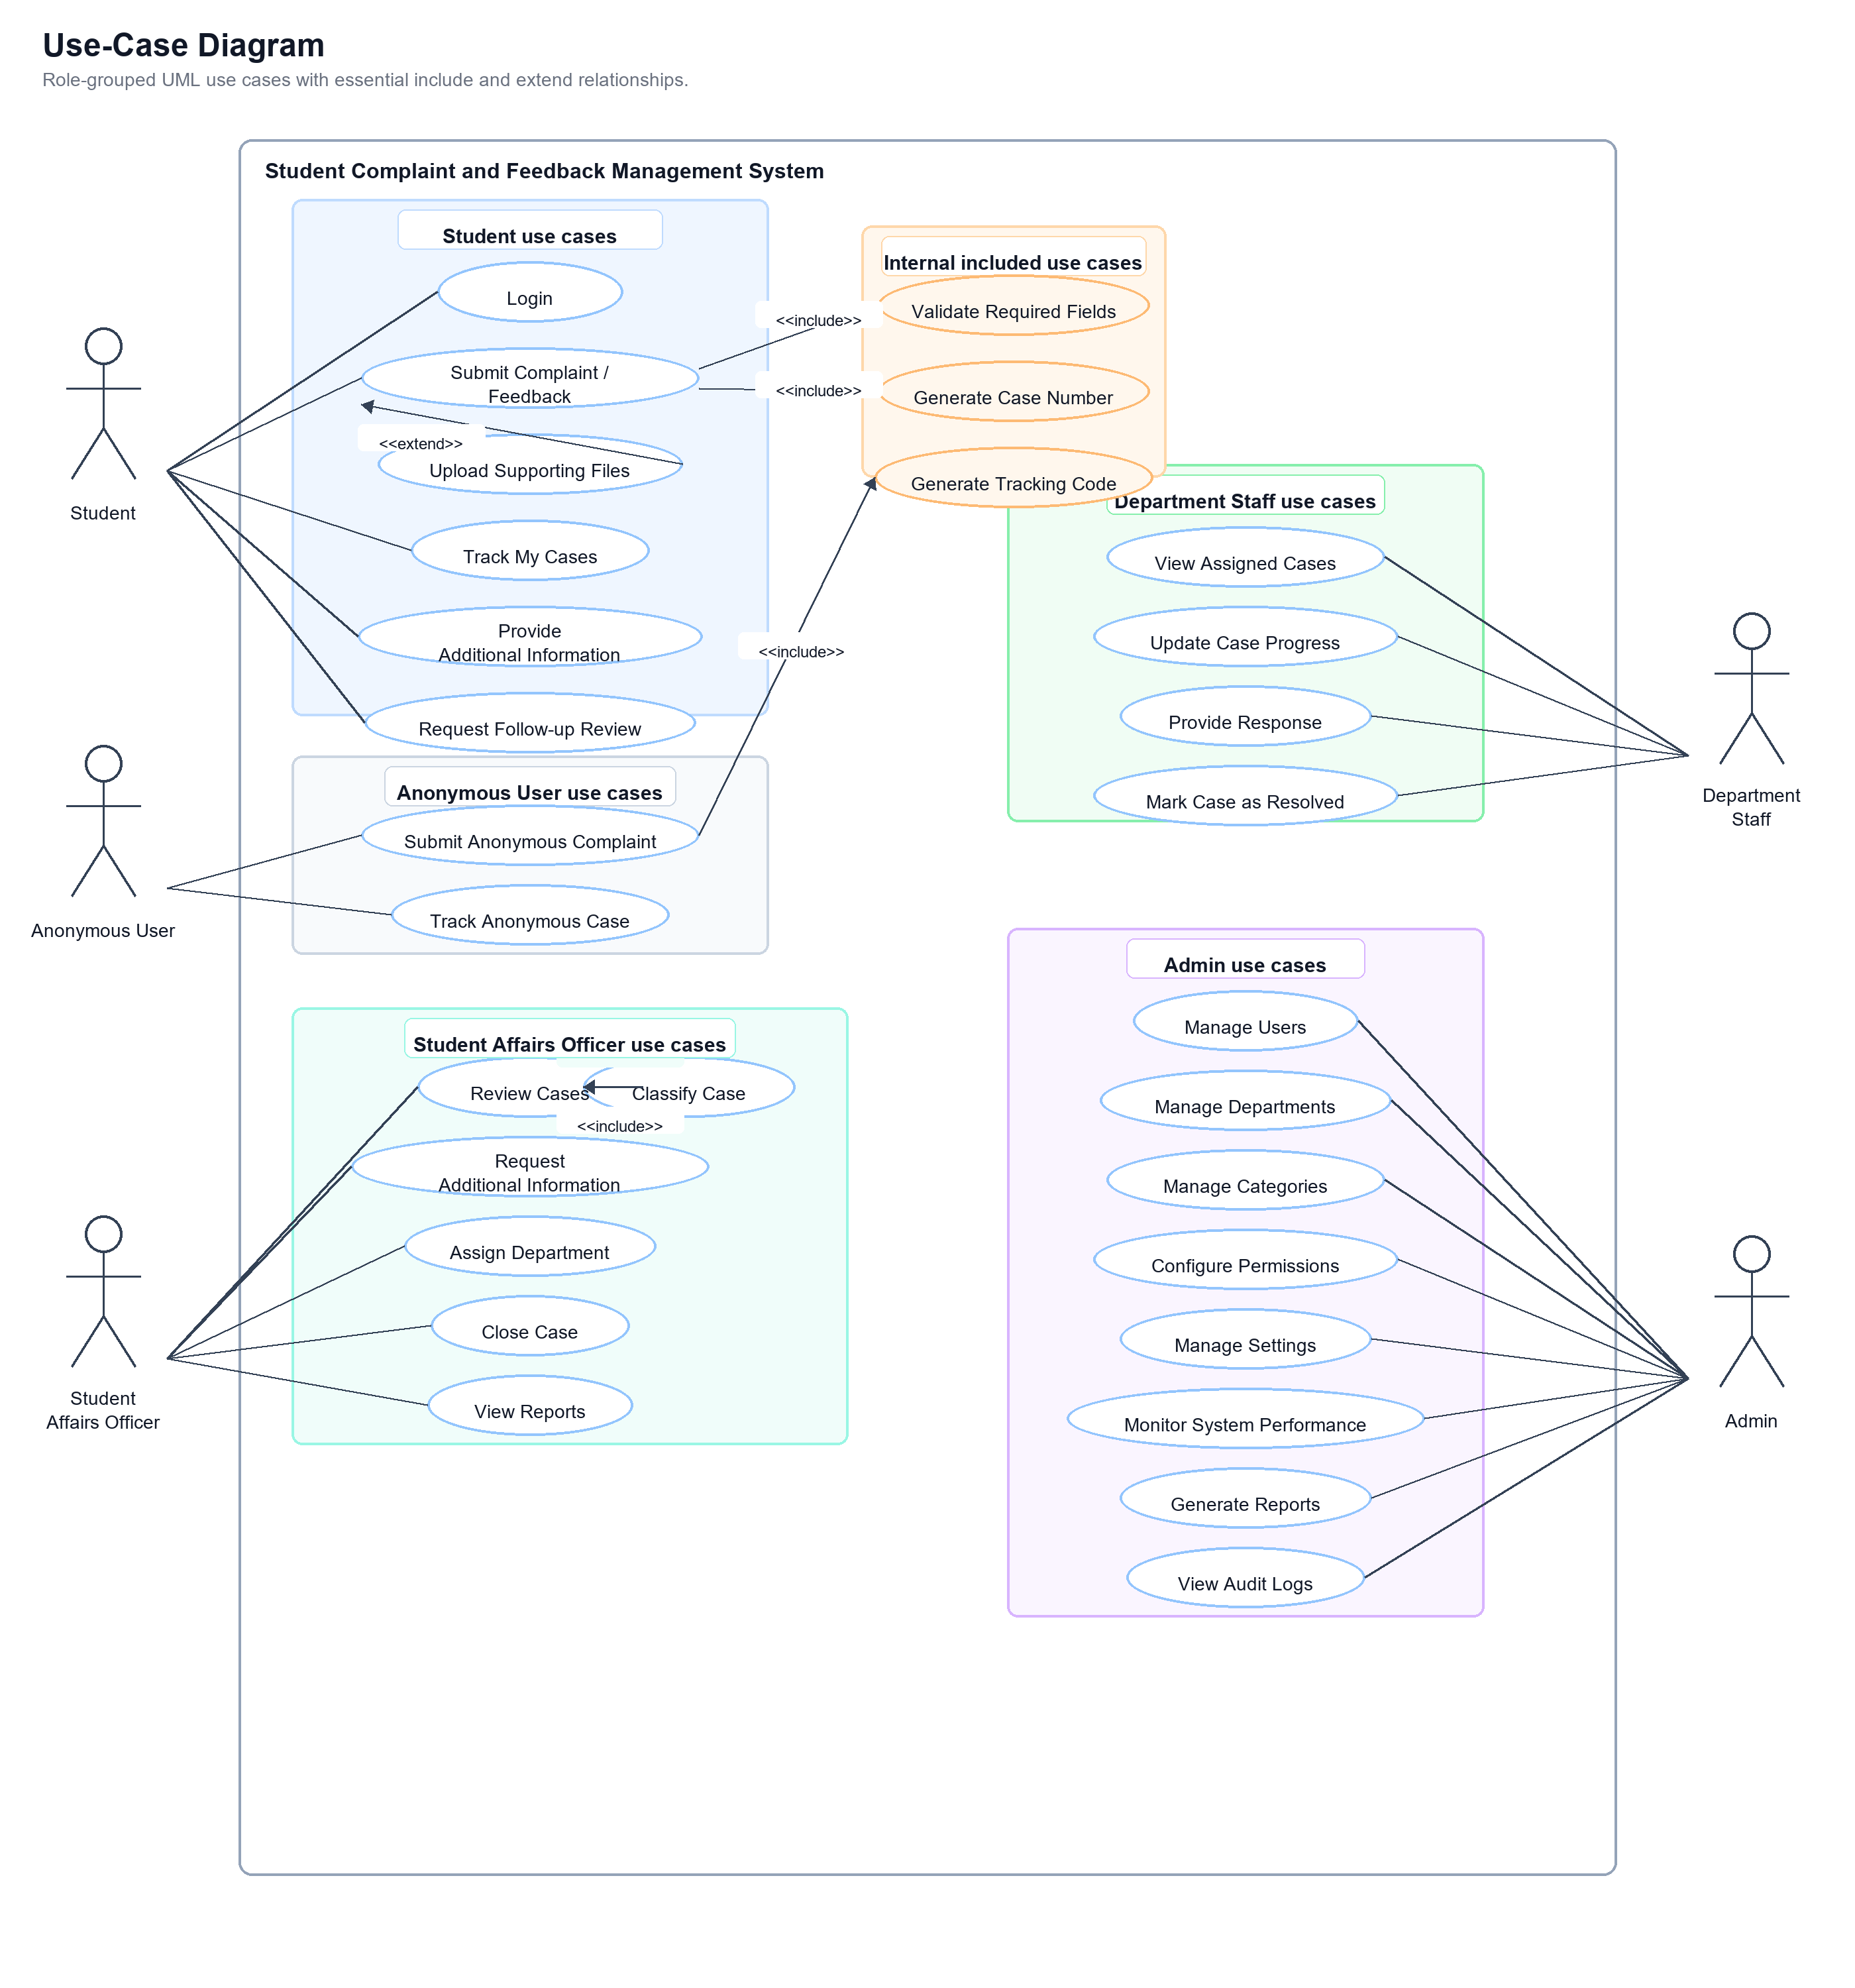
\includegraphics[width=0.94\textwidth,height=0.82\textheight,keepaspectratio]{figure2_use_case_diagram.png}
\caption{Use-case diagram for the complaint and feedback system.}
\label{fig:usecase}
\end{figure}

\subsection{UML class diagram}
The class diagram in \figref{fig:class} is the main OOAD model. \texttt{ComplaintCase} is the central class because most workflow records belong to a case. \texttt{User} represents login identity and role information. Student, Student Affairs Officer, Department Staff and Admin specialize the user role concept. \texttt{Category} controls classification, anonymous policy and default SLA. \texttt{Department} supports assignment. \texttt{CaseAttachment}, \texttt{CaseMessage}, \texttt{CaseStatusLog} and \texttt{CaseAssignment} are case-owned records.

The composition relationships from \texttt{ComplaintCase} to child records show that attachments, messages, status logs and assignments have no independent business meaning without a case. \texttt{Notification}, \texttt{AuditLog} and \texttt{SystemSetting} support cross-cutting behavior rather than the core case lifecycle. Although the diagram shows role specializations conceptually, the prototype implementation uses the \texttt{role} field in \texttt{User} for role-based access control. This model follows standard UML class notation and multiplicity concepts \cite{OMG2017UML}.

\begin{figure}[H]
\centering
  
\includegraphics[width=0.94\textwidth,height=0.74\textheight,keepaspectratio]{figure3_uml_class_diagram.png}
\caption{UML class diagram centered on \texttt{ComplaintCase}.}
\label{fig:class}
\end{figure}

\subsection{Activity diagram}
The activity diagram in \figref{fig:activity} explains the end-to-end complaint workflow with role labels indicating responsibility boundaries. It starts with case submission, continues through validation, case-number creation, anonymous handling, SLA log creation, notification, officer review, information request, department assignment, department processing, student review and case closure. The decision nodes represent "Need more info?" and "Satisfied?".

This diagram is important because the system is not only a data-entry form. It is a workflow system. The role labels show responsibility boundaries and help validate that each actor has a clear next action.

\begin{figure}[H]
\centering
  
\includegraphics[width=0.94\textwidth,height=0.82\textheight,keepaspectratio]{figure4_activity_diagram.png}
\caption{Activity flowchart for the complaint handling workflow.}
\label{fig:activity}
\end{figure}

\subsection{Sequence diagram}
The sequence diagram in \figref{fig:sequence} describes the complaint submission interaction. The user enters case details in the Vue frontend. The frontend includes authentication information when applicable and sends the request to the case API. Spring Security validates JWT-based access before the controller delegates the request to the case service. The service validates required fields, checks anonymous policy, saves attachments, persists the case and status log, and triggers notification creation. For anonymous cases, a tracking code is returned once.

The diagram demonstrates interaction design and responsibility allocation. Controllers handle HTTP boundaries, services enforce business rules, storage handles files, repositories persist data and the notification service communicates case events.

\begin{figure}[H]
\centering
  
\includegraphics[width=0.94\textwidth,height=0.74\textheight,keepaspectratio]{figure5_sequence_submission.png}
\caption{Sequence diagram for authenticated or anonymous complaint submission.}
\label{fig:sequence}
\end{figure}

\subsection{Entity relationship model}
The ER diagram in \figref{fig:er} shows the relational data model. It uses standard conceptual database-design concepts for entities, attributes, keys and relationships \cite{Elmasri2016Database}. The central \texttt{cases} table links to users, departments, categories and workflow child tables. Supporting tables store private notes, notifications, audit logs, weekly reports and settings.

The design separates reference data from workflow data. \texttt{departments} and \texttt{categories} are configurable reference tables. \texttt{case\_status\_logs}, \texttt{case\_messages} and \texttt{case\_assignments} preserve traceability. This structure supports both operational workflow and later reporting.

\begin{figure}[H]
\centering
  
\includegraphics[width=0.94\textwidth,height=0.82\textheight,keepaspectratio]{figure6_er_diagram.png}
\caption{Entity relationship diagram for the database design.}
\label{fig:er}
\end{figure}

\subsection{Role-based navigation}
The role navigation diagram in \figref{fig:navigation} translates system functions into frontend structure. It ensures that each actor sees only relevant menu items. This improves usability and also reinforces access-control thinking: students should not see officer tools, department staff should focus on assigned department work, and admins should access configuration and audit functions.

\begin{figure}[H]
\centering
  
\includegraphics[width=0.94\textwidth,height=0.74\textheight,keepaspectratio]{figure7_role_based_navigation.png}
\caption{Role-based frontend navigation structure.}
\label{fig:navigation}
\end{figure}

\section{System Evaluation and Testing}

\subsection{Functional testing}
The backend was tested with Maven and JUnit. The command \texttt{mvn test} completed successfully with 12 tests, 0 failures, 0 errors and 0 skipped tests. The tested areas included case notification flow, category policy, profile service, settings service, SLA policy, tracking code service and case number generation.

The frontend was tested with Vitest. The command \texttt{npm test} completed successfully with 8 test files and 20 tests passed. The tested areas included notification presentation, role home presentation, case presentation, dashboard presentation, authentication presentation, UI presentation, advanced presentation and API helper behavior.

\begin{table}[H]
\centering
\small
\begin{tabularx}{\textwidth}{p{0.18\textwidth}p{0.18\textwidth}p{0.18\textwidth}Y}
\toprule
Layer & Command & Result & Evidence\\
\midrule
Backend & \texttt{mvn test} & 12/12 passed & JUnit and Spring Boot tests validated service logic, policy behavior and workflow notifications.\\
Frontend & \texttt{npm test} & 20/20 passed & Vitest tests validated role-specific presentation, dashboard summaries, notifications, authentication and API utilities.\\
\bottomrule
\end{tabularx}
\caption{Automated test results recorded on June 6, 2026.}
\end{table}

\subsection{User testing and validation of requirements}
User testing was performed as scenario-based validation rather than large-scale production testing. The main scenarios were: student registration and login, authenticated case submission, anonymous submission, officer review, information request, department assignment, department progress update, resolution, follow-up review, admin configuration and report inspection. These scenarios validate the functional requirements in Section 3.

The testing approach follows the general purpose of software testing: checking that the implemented system satisfies specified requirements, reveals defects and supports intended use \cite{ISO29119Testing}. The prototype met the core course-project requirements, but additional formal user acceptance testing would be required before real university deployment.

\subsection{Performance observations}
The prototype is suitable for local demonstration and small course-project workflows. H2 supports quick local testing, while MySQL is available for deployment. The current system should not be presented as a production system for thousands of concurrent users because the free deployment plan, local file storage and external email limitations are not designed for that scale.

\subsection{Limitations and development challenges}
\begin{itemize}
  \item University SSO is not integrated; local database accounts are used instead.
  \item Local file upload is acceptable for demonstration but should be replaced by object storage in production.
  \item Email sending depends on SMTP or Resend configuration and may fail in free cloud environments.
  \item Anonymous tracking is designed for prototype use; stronger legal, privacy and abuse-prevention controls would be required for a real reporting platform.
  \item The report dashboard is useful for basic management, but advanced BI, trend analysis and root-cause analysis are future extensions.
\end{itemize}

\section{Achievement of Objectives and Conclusion}

\subsection{Summary of completed work}
The project completed a full-stack prototype of a student complaint and feedback management system. It includes a Spring Boot backend, Vue frontend, role-based access control, complaint submission, anonymous tracking, attachment support, officer review, department processing, notifications, audit logs, weekly reports and administration tools. The system was also documented with original OOAD and UML diagrams.

\subsection{Comparison between objectives and outcomes}
\begin{table}[H]
\centering
\small
\begin{tabularx}{\textwidth}{p{0.42\textwidth}p{0.18\textwidth}Y}
\toprule
Objective & Outcome & Evidence\\
\midrule
Role-based access for main actors & Achieved & Roles implemented in backend security and frontend navigation.\\
Authenticated and anonymous complaint submission & Achieved & Student and public case APIs, anonymous policy and tracking code service.\\
Officer and department workflow & Achieved & Officer and department controllers, services and workflow entities.\\
Notifications and auditability & Achieved & Notification, audit log and status log entities and services.\\
Reports and administration & Achieved & Admin user, reference, settings and weekly report functions.\\
OOAD documentation & Achieved & Architecture, use-case, class, activity, sequence, ER and navigation diagrams.\\
Prototype deployment pathway & Partially achieved for prototype deployment only & Deployment path exists for demonstration, but production-level readiness is not claimed.\\
\bottomrule
\end{tabularx}
\caption{Objective-outcome comparison.}
\end{table}

\subsection{Data and source artifacts availability}
Following the transparency logic of modern data-availability statements and FAIR principles \cite{Wilkinson2016FAIR,SpringerNatureDataPolicy}, the report, source code and demonstration materials are maintained in the project repository at \url{https://github.com/xuzihao723/StudentComplaintAndManagementSystem}. The report figures are included directly in this PDF, and the LaTeX source, PDF output and reference verification list are stored with the project documentation files. No real student complaint data are included in this report. Any demonstration accounts or seeded records are synthetic and intended only for testing and presentation.

\subsection{Future improvements}
Future work should include university SSO integration, object storage for attachments, verified email domain configuration, stronger anonymous-reporting safeguards, automated escalation rules, advanced workflow configuration, richer analytics, backup and recovery scripts, monitoring, accessibility audit and formal user acceptance testing with actual student-service staff.

\subsection{Conclusion}
The project achieved its main aim: it provides a structured, role-based and traceable prototype for managing student complaints and feedback. More importantly, the design demonstrates the application of OOAD concepts through requirements analysis, UML modeling, relational data design, workflow modeling and test-based evaluation. The prototype is not a production guarantee, but it is a complete and defensible course-project implementation that can be extended toward a real campus service platform.

\begin{thebibliography}{9}
\bibitem{OMG2017UML}
Object Management Group. Unified Modeling Language 2.5.1. OMG Specification, 2017. Available at: \url{https://www.omg.org/spec/UML/2.5.1}.

\bibitem{ISO29148}
ISO/IEC/IEEE. ISO/IEC/IEEE 29148:2018, Systems and software engineering: Life cycle processes: Requirements engineering. 2018. Available at: \url{https://www.iso.org/standard/72089.html}.

\bibitem{ScrumGuide2020}
Schwaber, K. and Sutherland, J. The Scrum Guide: The Definitive Guide to Scrum. 2020. Available at: \url{https://scrumguides.org/docs/scrumguide/v2020/2020-Scrum-Guide-US.pdf}.

\bibitem{Elmasri2016Database}
Elmasri, R. and Navathe, S. B. \textit{Fundamentals of Database Systems}, 7th edn. Pearson, 2016. Available at: \url{https://www.pearson.com/en-gb/subject-catalog/p/fundamentals-of-database-systems-global-edition/P200000004142/9781292097626}.

\bibitem{DatabaseConcepts2019}
Silberschatz, A., Korth, H. F. and Sudarshan, S. \textit{Database System Concepts}, 7th edn. McGraw-Hill, 2019. Available at: \url{https://codex.cs.yale.edu/avi/db-book/}.

\bibitem{ISO29119Testing}
ISO/IEC/IEEE. ISO/IEC/IEEE 29119-1:2022, Software and systems engineering: Software testing: Part 1: General concepts. 2022. Available at: \url{https://www.iso.org/standard/81291.html}.

\bibitem{Wilkinson2016FAIR}
Wilkinson, M. D. et al. The FAIR Guiding Principles for scientific data management and stewardship. \textit{Scientific Data} \textbf{3}, 160018 (2016). \url{https://doi.org/10.1038/sdata.2016.18}.

\bibitem{SpringerNatureDataPolicy}
Springer Nature. Research data policy. Accessed June 6, 2026. Available at: \url{https://www.springernature.com/gp/authors/research-data-policy}.
\end{thebibliography}

\end{document}
